    \documentclass[conference]{IEEEtran}
    
    \usepackage{graphicx}
    \usepackage{biblatex}
    \usepackage{multicol}
    \usepackage[utf8]{inputenc}
    \usepackage{xepersian}
    
    \bibliographystyle{ieeetr-fa}
    \settextfont{Gandom.ttf}
    \addbibresource{bib.bib}
    \renewcommand{\thesection}{\arabic{section}}
    \usepackage{blindtext, graphicx}
    \hyphenation{op-tical net-works semi-conduc-tor}
    
    \usepackage{blindtext, graphicx}
    
    \title{دسته بندی اتوماتیک ژانر موسیقی   }
    \author{
    امیر حسین باقری\\
    مصطفی لسانی\\
    حسین کافی
    }
    \date{پاییز 97}
    \renewcommand\footnoterule{\kern-3\hrule\kern2.6}
    
     
    
    \begin{document}
    \maketitle
    
    
    
    
    
    \section{مقدمه} 
    آهنگ ها، یکی از مهم ترین بخش های زندگی روزمره انسان ها می باشد. کمتر پیش می آید که ما روزانه دقایقی یا ساعتی از عمرمان را صرف گوش دادن به آهنگ ها نکنیم. یکی از مشکلاتی که بسیاری از ما هنگام گوش دادن به آهنگ ها پیدا می کنیم این است که الان با توجه به حس و حالی که در آن هستیم به چه آهنگی گوش دهیم.
    شرکت ها و سازمان های زیادی برروی این مشکل کار کرده اند و به راه حل های جالبی در این زمینه رسیده اند. اکثر آنها با پیاده سازی یک سیستم پیشنهاد دهنده آهنگ کار می کنند که بر دو اساس کار می کند: فیلتر کردن مشارکتی \LTRfootnote{ Collaborative filtering }   و  فیلتر مبنی بر محتوا \LTRfootnote{ Content-based filtering } . در سیستم فیلتر کردن مشارکتی، سیستم در مورد کاربر اطلاعاتی همچون علایق و سلایق را استخراج می کند و با توجه به اینکه کاربر های مشابه به چه آهنگ هایی گوش می دهند این آهنگ ها را به کاربر پیشنهاد می دهد. در مکانیزم فیلتر مبنی بر محتوا ، با استفاده از اطلاعات مربوط به آهنگ ها همچون ژانر، سال ، خواننده و غیره ، آهنگ های مشابه را پیدا کرده و به کاربران نشان می دهند. در هر دو مکانیزم اطلاعات زیادی نیاز است تا این سیستم به درستی کار کند. در حالت فیلتر مشارکتی به تعداد زیادی کاربر نیاز است که علایق آنها مشخص شده و در حالت فیلتر مبنی بر محتوا نیز اطلاعات زیادی هم چون ژانر آهنگ ، سالی که آهنگ انتشار یافت ، خواننده و غیره نیاز است. 
    در این مقاله با بررسی سیگنال های خام آهنگ و استفاده از الگوریتم های خوشه بندی ، آهنگ های همانند هم در یک خوشه قرار می گیرند. 
    ژانر ، برچسبی است که برای دسته بندی آهنگ های مشابه به کار می رود. اگر چه ژانر معمولا به صورت دستی توسط انسان ها مشخص می شود ، ما سعی داریم ژانر آهنگ ها را از طریق سیگنال خام آهنگ ها تخمین بزنیم. در این مقاله ما سیگنال آهنگ ها را بررسی کرده و ویژگی های خاصی که در آهنگ وجود دارد را استخراج می کنیم . سپس با استفاده از تکنیک های یادگیری ماشین آهنگ های مشابه را دسته بندی کرده و سپس بررسی می کنیم که چه مقدار این روش برای تشخیص درست ژانر آهنگ می تواند موثر باشد.
    \section{کار های مشابه}
    مطالعات زیادی در زمینه تشخیص ژانر آهنگ انجام شده است که از ویژگی‌های سیگنال آهنگ استفاده شده است. اغلب ساختار زمانی آهنگ \LTRfootnote {Temporal structure }   برای تشخیص ژانر به کار رفته است. از دنباله فعالیت واحد های پنهان و شبکه عصبی برای طبقه بندی به راک پاپ تکنو و کلاسیک استفاده کرد. از مدل پنهان مارکو  \LTRfootnote{ Hidden Markov model }    به همراه ویژگی استخراج شده از متد MFCCs  \LTRfootnote{ Mel-frequency cepstral coefficients }    برای خوشه بندی ژانر های پاپ کانتری جاز و کلاسیک استفاده کرد.
    برخی از روش‌ها تمرکز بر تشابه مستقیم بین ویژگی‌های استخراج شده از آهنگ دارند.
    با استفاده از بردار ویژگی آهنگ‌ها و فاصله میان این بردار ها درختی را تولید کرد تا به این طریق تشابه میان آهنگ‌های کلاسیک راک و جاز را نمایش دهد. با استفاده از روش خوشه بندی سلسله مراتبی اگلامورتیو به صورت ترتیبی آهنگ‌ها نزدیک به هم را در یک خوشه قرار داد 
    MFCCs که به مراتب در مطالعات استفاده شده است معیار خوبی از ویژگی‌های درون سیگنال آهنگ را به ما میدهد. این ویژگی‌ها بیشتر مناسب استخراج ویژگی مربوط به صحبت انسان است. از این رو مطالعات دیگر ویژگی‌های جدیدی را معرفی کردند مانند LPCs    \LTRfootnote{ Linear prediction coefficients }   و   RECCs  \LTRfootnote {Renyi Entropy Cepstral Coefficients }
    
    \section{ روش شناسی}
    \subsection{ انتخاب داده و استخراج ویژگی }
    20 آهنگ از هر ژانر کلاسیک  \LTRfootnote{ Classical }  , کانتری  \LTRfootnote{ Country } , متال  \LTRfootnote{ Metal }  , تکنو  \LTRfootnote{ Techno }  , چیل  \LTRfootnote{ Chill }  , اکوستیک  \LTRfootnote{ Acoustic }   و پانک  \LTRfootnote{ Punk }    انتخاب شده است. این آهنگ‌ها به طور رندم از اسپاتیفای انتخاب شده و هر آهنگ به طول 30 ثانیه می‌باشند. این داده‌ها بدون هیچ برچسبی به الگوریتم غیر نظارتی داده شده اند.
     برای استخراج ویژگی از هر یک از نمونه‌ها از چند روش استفاده کردیم
    \subsubsection{استخراج بیت \LTRfootnote{ Beat extraction }    آهنگ}
    کلمه بیت در لغت به معنای ضربان و یا ضرب در موسیقی می باشد که استفاده از آن در بین تنظیم کنندگان بسیار مرسوم است. بیت در موسیقی واژه‌ای است که قالبا به ریتم یک آهنگ گفته می‌شود. میانگین فاصله زمانی بین دو بیت به عنوان ویژگی از آهنگ استخراج شده است

    \subsubsection{ استخراج CENS \LTRfootnote{ Chroma Energy Normalized }     }
    در موسیقی ویژگی کروما ارتباط بسیار نزدیکی با ۱۲ نت موسقی دارد. استخراج ویژگی بر اساس کروما ابزار بسیار قدرتمندی را برای طبقه بندی بر اساس نت موسقی به ما می‌دهد. ویژگی اصلی کروما است است که ویژگی ملودیک و هارمونیک آهنگ را استخراج کند.
\begin{figure}[h!]
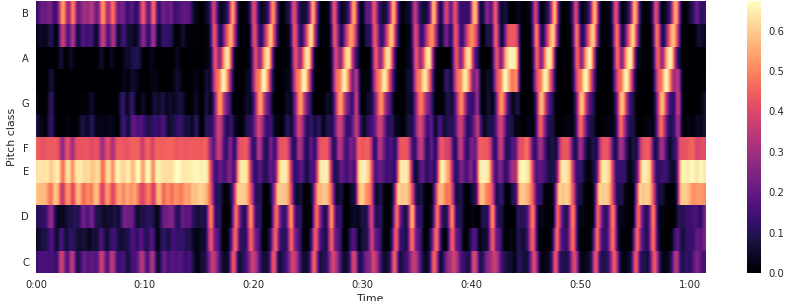
\includegraphics[width=\linewidth]{1.png}
      \caption{نمونه ای از ویژگی کروما استخراج شده از آهنگ }
      \label{fig:fig 1}
    \end{figure}
    \subsubsection{استخراج MFCCs}
    استفاده از ویژگی MFCCs  در سیستم‌های تشخیص صحبت \LTRfootnote{ Music information retrieval }  بسیار رایج است. از این ویژگی همچنین در  استخراج اطلاعات از آهنگ  \LTRfootnote{ Speech recognition system }  مانند طبقه بندی ژانر موسیقی نیز استفاده می‌شود. 
    نحوه استخراج این ویژگی به شکل زیر است
    \begin{itemize}
    \item  تبدیل فوریه سیگنال را محاسبه میکنیم.
    \item توان به دست آمده در طیف بالا را به mel scale نگاشت میدهیم.
    \item لگاریتم توان ها را در فرکانس مل  \LTRfootnote{ Mel frequencies }  محاسبه میکنیم. 
    \item تبدیل گسسته کسینوس را برای سیگنال به دست آمده محاسبه میکنیم. 
    \item دامنه هر یک از طیف ها, MFCCs می باشد.
    
    \end{itemize}
    \begin{figure}[h!]
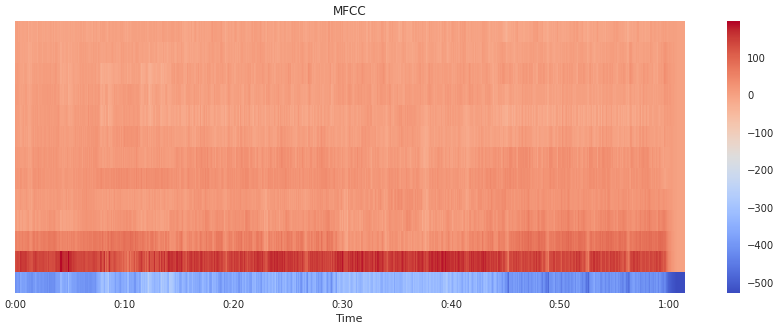
\includegraphics[width=\linewidth]{3.png}
      \caption{  ویژگی MFCCs }
      \label{fig:fig 1}
    \end{figure}

    \subsubsection{ طیف سنجی بر اساس مرکز \LTRfootnote{ Spectral Centroid }     }
طیف سنجی بر اساس مرکز مقیاسی است که در پردازش سیگنال دیجیتالی برای توصیف کردن طیف به کار می‌رود. این مقیاس مشخص میکند مرکز ثقل طیف در کجا قرار دارد. نمونه‌ای از این ویژگی را در شکل زیر میبینید. 
    \begin{figure}[h!]
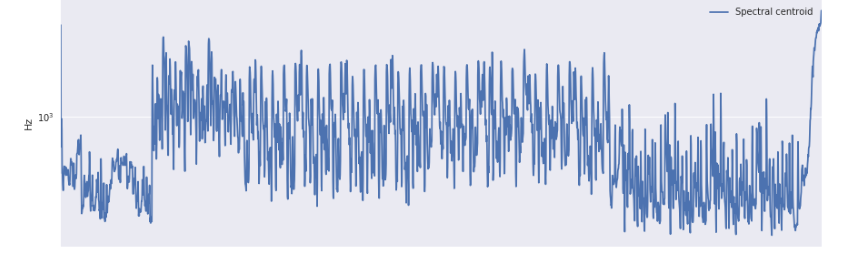
\includegraphics[width=\linewidth]{4.png}
      \caption{  Spectral Centroid
}
      \label{fig:fig 1}
    \end{figure}


    \subsubsection{ طیف سنجی بر اساس تضاد  \LTRfootnote{ Spectral Contrast }     }
طیف سنجی بر اساس تضاد نیز برای توصیف آهنگ توسعه یافت. این ویژگی, قله و دره را در هر زیر باند به طور جدا گانه در نظر میگیرد. به طور کلی, قله طیف نمایانگر جز هارمونیک و دره طیف نمایانگر بخش غیر هارمونیک یا نویز می‌باشد. بنابراین تفاوت میان قله طیف و دره طیف, بازتاب توزیع تضاد موجود در طیف است. نمونه‌ای از این ویژگی را در شکل زیر میبینیم. 

    \begin{figure}[h!]
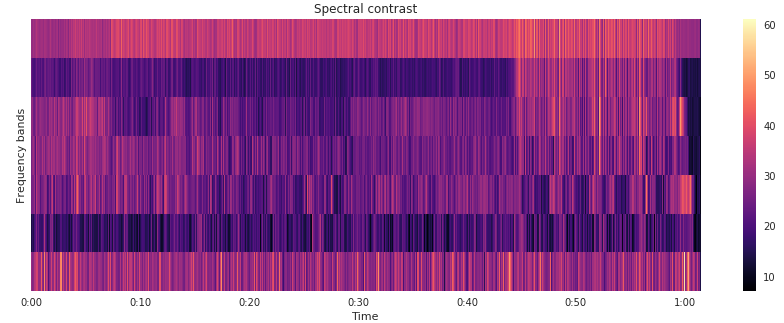
\includegraphics[width=\linewidth]{5.png}
      \caption{  Spectral Contrast
}
      \label{fig:fig 1}
    \end{figure}

\subsubsection{ استخراج نرخ عبور از صفر
  \LTRfootnote{ Zero Crossing Rate }     }
نقطه عبور از صفر نقطه‌ای است که دامنه سیگنال در در آن نقطه صفر است. در نقاط دیگر, دامنه  موج یا به سمت قله می‌رود یا به سمت دره نزول میکند. 
نرخ عبور از صفر, نرخی است که مقدار سیگنال در آن مثبت و منفی می‌شود یا بر عکس. این ویژگی به طور مکرر در تشخیص صدا و استخراج اطلاعات از آهنگ استفاده می‌شود.

    \begin{figure}[h!]
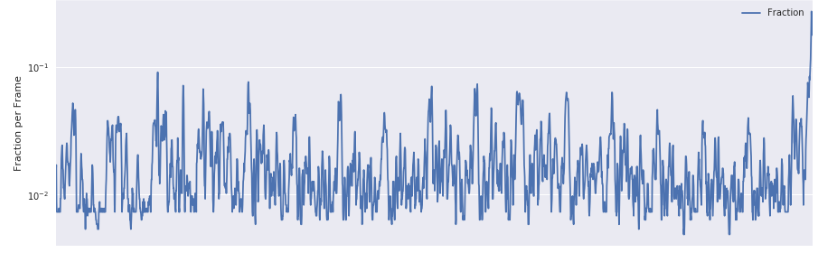
\includegraphics[width=\linewidth]{6.png}
      \caption{  Zero Crossing Rate 

}
      \label{fig:fig 1}
    \end{figure}


\begin{thebibliography}{99}
\begin{LTRbibitems}

\bibitem{1}
Soltau, H., Schultz, T., Westphal, M., Waibel, A. (1998).
Recognition of music types. In Acoustics, Speech and
Signal Processing, 1998. Proceedings of the 1998 IEEE
International Conference on (Vol. 2, pp. 1137-1140).
IEEE.

\bibitem{2}
Shao, X., Xu, C., Kankanhalli, M. S. (2004). Unsupervised
classification of music genre using hidden markov model.
In Multimedia and Expo, 2004. ICME’04. 2004 IEEE
International Conference on (Vol. 3, pp. 2023-2026).
IEEE.

\bibitem{3}
Cilibrasi, R., Vitányi, P., De Wolf, R. (2004). Algorith-
mic clustering of music based on string compression. In
Computer Music Journal on (Vol.28, no. 4, pp. 49-67).
IEEE.
\bibitem{4}
Tsai, W.H., Bao, D.F. (2010). Clustering music recordings
based on genres. In Information Science and Applications
(ICISA), 2010 International Conference on (pp. 1-5).
IEEE.
\bibitem{5}
Peng, W., Li, T., Ogihara, M. (2007). Music Clustering
with Constraints. In ISMIR (pp. 27-32).


\end{LTRbibitems}
\end{thebibliography}
 
    
    \end{document}

